\documentclass[12pt]{article}
\setlength{\oddsidemargin}{0in}
\setlength{\evensidemargin}{0in}
\setlength{\textwidth}{6.5in}
\setlength{\parindent}{0in}
\setlength{\parskip}{\baselineskip}

\usepackage{amsmath,amsfonts,amssymb,graphicx,enumerate}

\begin{document}

CSCI 5454 \hfill Problem Set 2\\
Robert Werthman\\
Collaborators: Swapnil Paratey 

\hrulefill

\begin{enumerate}

	\item \textit{Probability boot camp}
	
	\begin{enumerate}
	
		\item \textit{Prove Markov's inequality, $Pr[X \ge c] \le E[X]/c$, with $c>0$}\\
		\\
		The formula for the probability of a continuous random variable $X$ with probability density function $f(x)$ is
			$$
			Pr[x_1 \le X \le x_2] = \int_{x_1}^{x_2} f(x)dx
			$$	
		And the formula for the expected value of a continuous random variable $X$ with probability density function $f(x)$ is
			$$
			E[x_1 \le X \le x_2] = \int_{x_1}^{x_2} xf(x)
			$$	
		so for $Pr[X \ge c]$ we have
			$$
			Pr[X \ge c] = \int_{c}^{\infty} f(x)dx
			$$
		and since $X$ is a nonnegative random variable we have
			$$
			E[X] = \int_{0}^{\infty} xf(x)dx
			$$
		Notice that $0 < c \le \infty$.  This tells us that the bounds of $E[X]$ are greater than $Pr[X \ge c]$.  We can break up the integral formed by $E[X]$ to create an inequality that 
		will begin to look similar to the integral of $Pr[X \ge c]$.
			\begin{align*}
				E[X] &= \int_{0}^{\infty} xf(x)dx\\
				&= \int_{0}^{c} xf(x)dx + \int_{c}^{\infty} xf(x)dx\\
				&\ge \int_{c}^{\infty} xf(x)dx\\
			\end{align*}
		We can assume that $x \ge c$ because $c$ is one of the bounds of the integral.  This means we can substitute $c$ for $x$.
			\begin{align*}
				 \int_{c}^{\infty} xf(x)dx \ge \int_{c}^{\infty} cf(x)dx \ge c\int_{c}^{\infty} f(x)dx
			\end{align*}
		We now have an equation for $E[X]$ that has $Pr[X \ge c]$.
			$$
			E[X] \ge c\int_{c}^{\infty} f(x)dx = cPr[X \ge c]
			$$
		Dividing both sides by $c$ gives us
			$$
			E[X]/c \ge Pr[X \ge c]
			$$
		which is Markov's inequality.  We have just shown that $Pr[X \ge c] \le E[X]/c$, with $c>0$ is true based on the probability and expected value of the continuous random variable $X$.
		
		\newpage
		\item \textit{Prove Chebyshev's inequality $Pr[|X-\mu| \ge c \cdot \sigma] \le 1/c^2$}\\
		\\
		If we let $k = (c \cdot \sigma)$ we have
			$$
			Pr[|X-\mu| \ge c \cdot \sigma] = Pr[|X-\mu| \ge k]
			$$
		One of the properties of $|a|$ is that it can also be represented as $\sqrt{a^2}$ so we can change\\
			$$
			Pr[|X-\mu| \ge k] = Pr[\sqrt{(X-\mu)^2} \ge k]
			$$
		If we take the square root of both sides of the inequality we get
			$$
			Pr[(X-\mu)^2 \ge k^2]
			$$
		From here we can use Markov's inequality since we know $(X-\mu)^2$ is nonnegative.  If we let $(X-\mu)^2 = X$ and $k^2 = c$ and substitute those into Markov's inequality we have 
			$$
			Pr[(X-\mu)^2 \ge k^2] \le E[(X-\mu)^2]/k
			$$
		The variance $\sigma^2$ of a continuous random variable $X$ with mean $\mu$ is 
			$$
			\sigma^2 = E[(X-\mu)^2]
			$$
		So
			$$
			Pr[(X-\mu)^2 \ge k^2] \le E[(X-\mu)^2]/k
			$$
		Now becomes
			$$
			Pr[(X-\mu)^2 \ge k^2] \le \sigma^2/k
			$$
		If we now change $k$ back to $c \cdot \sigma$ we have the equation
			$$
			Pr[(X-\mu)^2 \ge (c \cdot \sigma)^2] \le \sigma^2/c^2 \cdot \sigma^2
			$$
		Reducing the right side of the equation results in
			$$
			Pr[(X-\mu)^2 \ge (c \cdot \sigma)^2] \le 1/c^2
			$$
		And taking the square root of both sides of the inequality on the left hand side of the equation results in
			$$
			Pr[\sqrt{(X-\mu)^2} \ge c \cdot \sigma] \le 1/c^2
			$$ 
		
		Which can be further reduced to 
			$$
			Pr[|X-\mu| \ge c \cdot \sigma] \le 1/c^2
			$$ 
		Which is Chebyshev's inequality.  We have just shown that Chebyshev's inequality can be proven using Markov's Inequality.
		\newpage
		\item \textit{Show that for any discrete random variables $X,X',E[X] = E[E[X|X']]$.}\\
		\\
		If we let $Y = X'$ we have
			$$
			E[X] = E[E[X|Y]]
			$$
		The expected value of a discrete random variable X is
			$$
			E[X] = \sum_{x} x \cdot Pr[X=x]
			$$
		The conditional probability for any two discrete random variables $X,Y$ is defined to be 
			$$
			Pr[X=x|Y=y] = \frac{Pr[X=x \cap Y=y]}{Pr[Y=y]}
			$$
		The conditional expectation for any two discrete random variable $X,Y$ is defined to be
			$$
			E[X|Y=y] = \sum_{x} x \cdot Pr[X=x|Y=y]
			$$
		Given the above assertions the proof is with the help of online sources \cite{4,5,6}
			\begin{align*}
				E[E[X|Y]] &= E[\sum_{x} x \cdot Pr[X=x|Y]]\\
				&=\sum_{y} [\sum_{x} x \cdot Pr[X=x|Y=y]] \cdot Pr[Y=y]\\
				&=\sum_{x} x \sum_{y} Pr[X=x|Y=y] \cdot Pr[Y=y]\\
				&=\sum_{x} x \cdot Pr[X=x]\\
				&=E[X]
			\end{align*}
		
		\newpage
		\item \textit{Prove by induction that $E[X_t] = 0$ for a martingale.}\\
		\\
		We want to show that in a martingale sequence the expected value for a random variable $X_{t+1}$ is the random variable $X_t$ before it.\\
		\\
		\textbf{Base case: }\\
		\\
		When $t=0$ with $X_0 = 0$ we have
			\begin{align*}
			E[X_1|X_0] &= \sum_{x} x \cdot Pr[X_1=x|X_0 = 0]\\
			&=0\\
			\end{align*}
		\textbf{Inductive step: }\\
		\\
		We showed that the base case $E[X_1|X_0] = 0$ is true.  Therefore, we can say that $E[X_2|X_1] = E[E[X_1|X0]] = 0$ no matter what $X_2$ is.   This leads to the equation
			$$
			E[X_t|X_0,...,X_{t-1}] = E[E[...E[X_{1}|X_{0}]]] = 0
			$$
		So by induction we have just shown that $E[X_t] = 0$.
		
	\end{enumerate}
	\newpage
	\item \textit{Give a graph $G$ with a source vertex $s$ and a set of edges $E_\pi$ to every vertex in $G$ such that the path from $s$ to $v$ is the shortest
	path but the set of the edges $E_\pi$ cannot be produced by running a breadth-first search on $G$.} \\
	\\
	\begin{figure}[h]
	\caption{Example of a graph where there exists a set of edges that are the shortest path between vertices but will not be found by a breadth first search.}
	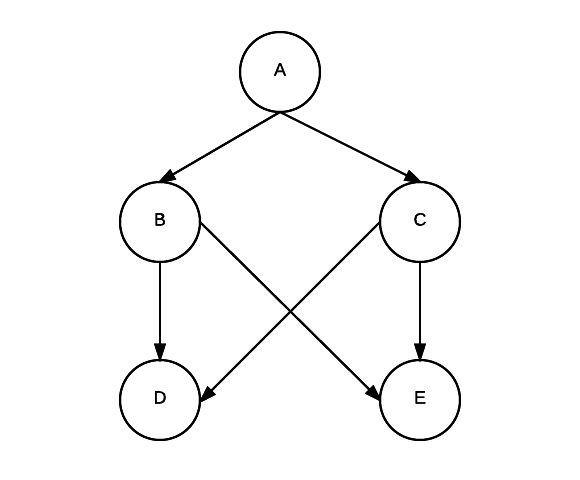
\includegraphics[width=6cm]{ps2_q2.png}
	\centering
	\end{figure}
	\\
	For this question, the shortest-path from $s$ to $v$ is defined as the minimum number of edges in any path from vertex $s$ to vertex $v$.  
	If we let the source vertex $s$ be vertex $A$ then the set of edges $E_\pi$ that cannot be produced by running a breadth first search are
	$$
	\{(A,B),(A,C),(B,D),(C,E)\}
	$$
	This is the case because of how breadth first search discovers vertices.  It starts at a source vertex $s$ and then adds every vertex in the adjacency list of $s$ to a queue.  
	In the case above $s$ will be $A$ and it will add $B$ and $C$ to the queue because those are the vertices adjacent to $A$.  
	An edge from $A$ to $B$ and from $A$ to $C$ will be created.  
	Once it does that it will then pop off the first vertex on the queue which will be either $B$ or $C$ depending on the ordering of the adjacency list of $A$.  
	It will then add every vertex from the adjacency list of the vertex is pops off to the queue.
	If either $B$ or $C$ is removed from the queue, $D$ and $E$ are still both added to the queue because there are both in $B$ and $C$ adjacency lists.
	In either case, edges are created from a single vertex, $C$ or $B$, to both $D$ and $E$ i.e. $(C,D),(C,E)$.  It will never be the case that both $C$ and $B$ will have a only single edge i.e. $(C,D),(B,E)$.
	It will only be the case that one of them will have two edges so the set of edges $E_\pi$ above will would never occur with a breadth first search.
	\newpage
	\item \textit{Give an efficient algorithm with an input of a graph $G$ and and an edge $e$ and returns a cut where $e$ is a light edge across the cut or NO if no such cut exists}\\
	\\
	\textbf{Psuedocode}
	\begin{verbatim}
	def LightEdgeCut(G,e):
	    minimum spanning tree = Kruskal's algorithm
	    if e is in minimum spanning tree:
	        create a cut of the graph with e as a light edge
	        return cut
	    else:
	        add e to minimum spanning tree to create a cycle C
	        z = largest edge removed from cycle C
	        if z is e: // Cycle property of minimum spanning tree
	            return NO
	        else:
	            create a cut of the graph with e as a light edge
	            return cut
	\end{verbatim}
	
	\textbf{Correctness}\\
	\\
	The algorithm above depends on two assumptions:
	\begin{enumerate}
		\item If an edge $(u, v)$ is contained in some minimum spanning tree, then it is a light edge crossing some cut of the graph \cite{2}.
		\item For any cycle C in the graph, if the weight of an edge e of C is larger than the individual weights of all other edges of C, then this edge cannot belong to a MST \cite{3}.
	\end{enumerate}
	As an example for hypothesis (a) we cut the the graph of Figure 2 between vertices $A$ and $D$ and vertices $D$ and $E$.  After the cut $S = \{D\}$ and $S'=\{A,B,C,E,F\}$.
	The edge $(A,D)$ is in the minimum spanning tree created by Kruskal's algorithm and it is a light edge of the cut that was made.\\
	\\
	As an example for hypothesis (b) if we add the edge $(D,E)$ to the minimum spanning tree it will create a cycle from vertices $A \rightarrow B \rightarrow E \rightarrow D \rightarrow A$.
	If we remove the largest weighted edge which in this case we say is $(A,D)$ even though it is the same weight as $(D,E)$ we get a new minimum spanning tree that has $(A,D)$ as an edge.  
	If $(A,D)$ had been larger than $(D,E)$ then it would have been removed from the minimum spanning tree and would not be part of any other minimum spanning tree.\\
	\\ 
	We assume Kruskal's algorithm is correct and returns a minimum spanning tree for the graph $G$.  
	It may be that the edge $e$ LightEdgeCut takes as input is part of the minimum spanning tree returned by Kruskal's algorithm.  
	We then know that the edge $e$ is a light edge crossing some cut of $G$ so we can create that cut with $e$ and return it. \\
	\\ 
	If $e$ is not in the minimum spanning tree returned by Kruskal's algorithm then we have to check to see if $e$ is part of any minimum spanning tree of $G$.
	We do this by adding it to the minimum spanning tree returned by Kruskal's algorithm in order to create a cycle.  
	Based on the cycle property of minimum spanning trees the largest edge in a cycle cannot be part of any minimum spanning tree.  If $e$ is the largest edge
	in the cycle we know it is not part of a minimum spanning tree and therefore not a light edge crossing some cut of the graph.  If it is not the largest edge then
	we can conclude it is part of a minimum spanning tree and is a light edge crossing some cut of the graph.\\
	\begin{figure}[h]
	\caption{A graph where the edges of a minimum spanning tree created by Kruskal's algorithm are highlighted in green.}
	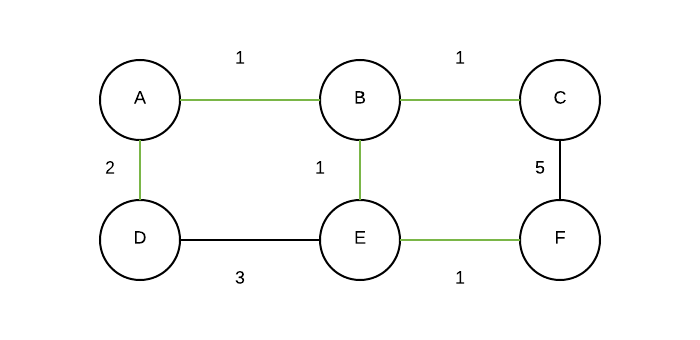
\includegraphics[width=8cm]{ps2_q3.png}
	\centering
	\end{figure}
	\\
	\textbf{Runtime}\\
	\\
	Kruskal's algorithm runs in $O(V\,log(E))$.  The worse case of this algorithm will, after going through Kruskal's algorithm, go to the else statement.
	Assuming the minimum spanning tree is a disjoint-set data structure adding the edge $e$ to the spanning tree is a set union operation that takes $O(1)$.
	Finding the edge with the highest weight in the cycle could take $O(V-1)$ if the cycle contains all of the edges in the minimum spanning tree.
	Checking if the largest edge is $e$ takes $O(1)$.  
	Creating a cut of the graph $G$ with $e$ as a light edge takes O(V) if it has to look at all of there vertices where to make the cut.
	The worst case runtime would be $O(V\,log(E)+V+(V-1)) = O(V\,log(E) + V)$.\\
	
	\newpage
	\item \textit{Give a $o(|V|^2)$ algorithm to find a universal sink given an adjacency matrix.}\\
	\\
	\textbf{Pseudocode}
	\begin{verbatim}
	FindUniversalSink(A):
	 for k in range(1,|V|):
	  vertex k is a universal sink
	  for i in range(1,|V|):
	   if i != k and A_{ik} == 0: // 0 in the vertex's column that is not a self loop 
	    vertex k not universal sink
	    break
	  for j in range(1,|V|):
	   if A_{kj} == 1: // 1 in the vertex's row
	    vertex k not universal sink
	    break
	 if vertex k is still a universal sink:
	  return vertex k
	 elif k == |V|:
	  return NO
	\end{verbatim}
	\textbf{Correctness}\\
	\\
	In order for this algorithm to be correct I make the following assumptions about an adjacency matrix:
	\begin{enumerate}
		\item If a graph is represented as an adjacency matrix $A$ then $A_{ij}$ is the edge from vertex $i$ to vertex $j$. \\ 
		\item If a 1 is present in the matrix at row $i$ column $j$ then an edge exists from $i$ to $j$.  If a 0 is present then no edge exists from $i$ to $j$.\\
		\item A universal sink will have 0's in its entire row of the adjacency matrix meaning there are no edges from it to any other vertex or to itself in the form of a self-loop.\\  
		\item Every vertex, not including the universal sink, will have a 1 in the column the belongs to the universal sink.  This means that they all have edges from themselves to the universal sink.\\
		\item A vertex that has a 1 in any part of its row in the matrix or a 0 in any part of its column in the matrix other then the cell that is a self-loop then it is not a universal sink.\\
	\end{enumerate}
	I claim that FindUniversalSink will always return a universal sink if there is one to be found in the adjacency matrix $A$ otherwise NO is returned.  
	It does this by looking at and assuming every vertex in the adjacency matrix is the universal sink until proven otherwise.\\
	\\
	The algorithm begins with a adjacency list.  It continues by iterating vertex by vertex through the adjacency list, setting each vertex as the universal sink.  
	Each time a new vertex is set as the universal sink it first looks at the entire column of the vertex and checks to see if there is a 0 in any place other than the self loop cell where row number $i$ equals column number $j$.     
	This indicates this vertex is not a universal sink because it does not have an edge from every other vertex in the graph going to it.
	The algorithm then looks at the row of the vertex to see if there are any 1's in any place.  This also indicates this vertex is not a universal sink because a universal sink does not have any out-edges.
	If it is found that this vertex is not a universal sink by either looking at the column or the row of the vertex, the algorithm sets the vertex to not being a universal sink and breaks out of whichever loop it is currently and 
	ends up at a conditional statement.\\
	\\
	This conditional statement checks if the vertex is still a universal sink.  If it is a universal sink the vertex is returned otherwise two things could happen.  
	We could be at the last vertex in the adjacency list which, if we have reached this point, is not a universal sink so there exists on universal sink the graph.
	Or we could not be at the last vertex in the adjacency list which means we will go back to the top loop and move to and check the next vertex in the adjacency list.
	
	\textbf{Runtime}\\
	Unfortunately, I was unable to to create an algorithm that had a runtime of $o(|V|^2)$.
	The first loop of FindUniversalSink runs from $|V|$ times as it goes through all of the vertices.  
	With in that loop, there are two other loops that also run through all of the vertices in the adjacency graph so they run a total of $2|V|$ times.
	The rest of the operations like checking the values in the cells of the matrix or seeing if a vertex is a universal sink run in in constant time.\\
	\\
	This means this algorithm has a runtime of $O(|V|*2|V|) = O(|V|^2)$.  
	
	\newpage
	\item
		\begin{enumerate}
			\item \textit{Prove that every tree is a bipartite graph.}\\
			\\
			\begin{figure}[h]
			\caption{An example of a bipartite graph.}
			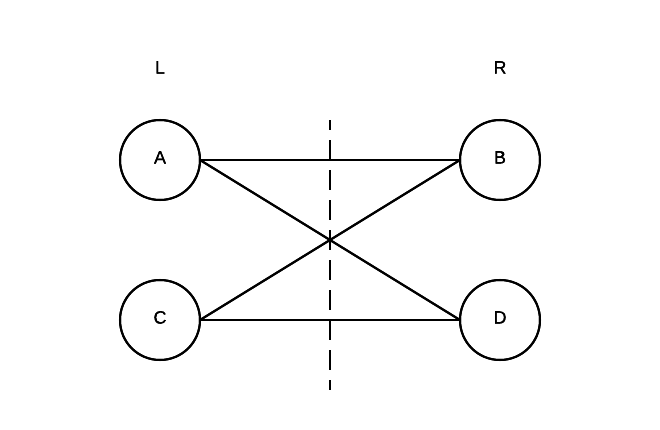
\includegraphics[width=8cm]{ps2_q5a.png}
			\centering
			\end{figure}
			\\
			\begin{figure}[h]
			\caption{An example of a non bipartite graph.}
			\includegraphics[width=8cm]{ps2_a5aa.png}
			\centering
			\end{figure}			
			\begin{figure}[h]
			\caption{An example of a tree.}
			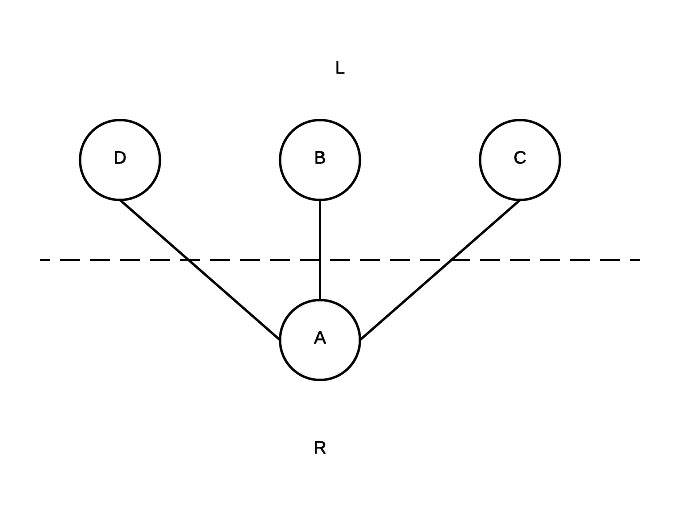
\includegraphics[width=8cm]{ps2_q5aaa.png}
			\centering
			\end{figure}
			\newpage
			If you notice in the pictures above a graph that has an even number of vertices in a cycle (an even cycle) is bipartite while a graph that has an odd number of vertices in a cycle (an odd cycle) is not bipartite \cite{1}.
			A tree is a connected, acyclic, and undirected graph.  Since it does contain any cycles, in particular an odd cycle, I claim it must be bipartite.\\
			\\
			If we were to assume a tree was not bipartite then no matter how the vertices were partitioned there would always be at least one edge $(u,v)$ of the tree where $u$ and $v$ were in the 
			same vertex subset if the vertices were broken into two susbets.  
			Starting with two vertices in a tree which is the minimum number of vertices to form an edge those vertices can be partitioned into two subsets that will make the tree bipartite.  
			The edge $(u,v)$ between the two vertices will have one end in one subset and the other end in the other subset.\\
			\\
			With three or more vertices in a graph, the only way to make a graph not bipartite is to create cycles between the vertices as in Figure 4.  But as we see in Figure 3, a graph with an even cycle is still bipartite.  
			This would mean a tree would need to have an odd cycle to not be bipartite but because a tree by definition will never have any cycles it will always be bipartite.\\    
			\newpage
			\item \textit{Given an efficient alogrithm to determine whether a given undirected graph is bipartite.}\\
			\\
			\textbf{Correctness}\\
			\\
			We can determine if an undirected graph is bipartite by coloring the vertices in the graph with two different colors \cite{7}.
			We can search through the graph and when we hit one endpoint of an edge we color it one color and when we hit the next endpoint of the edge we color it a different color.
			We will end up with all the nodes in $R$ being a different color compared to the color of all of the nodes in $L$ if the graph is bipartite.
			To do this we can use a modified breadth first search.\\
			\\
			When we run breadth first search we first take the source vertex that is in the input to the algorithm and color it one particular color--lets say red for this example.
			Then we put it on the queue.  When the source is removed from the queue we check to make sure its color is correct and then we look at all of its neighbors.  
			To figure out which color to use for the neighbors of any vertex we look at the distance from the the source vertex to each neighbor vertex.  
			In the example of the neighbors of the source vertex they will all be a distance of one away from the source so we color them green.  The next vertices from the source's neighbors will
			be a distance of two away so we will color them red.  To generalize, any vertex that is an even distance away is colored red and any vertex that is an odd distance away from the source
			will be colored green.  If we pop a vertex from the queue and check its color and it disagrees with the coloring scheme we know that this graph is not bipartite.\\			
			\\
			Since breadth first search discovers nodes one level of distance away from the source vertex at a time this change to the algorithm ensures 
			that if the graph is bipartite the vertices will be colored in a way that leaves each endpoint of an edge a different color.
			This means that vertices of color one can be partitioned into one subset $R$ and vertices of color two can be partition into another subset $L$.  
			These subsets will have one endpoint of an edge in $R$ and one endpoint of an edge in $L$.\\
			\\
			\textbf{Runtime}\\
			\\
			The regular breadth first search algorithm runs in $O(V+E)$.  
			We are adding a color attribute to a node which is just another array and inserting and checking the values of the array takes O(1) time per node.  
			I claim that the runtime of the modified breadth first search remains $O(V+E)$.
		\end{enumerate}
		
		\newpage
		\item
			\begin{enumerate}
				\item \textit{Give an example graph with a unique MST and two edges of equal length.  Give an algorithm to construct a graph with $\Omega{(|V|^2)}$
				edges of equal weight yet still having an unique MST.}\\
				\\
				\textbf{Example Graph}\\
				\\
				\begin{figure}[h]
				\caption{An example of a unique MST with two edges of equal length.}
				\includegraphics[width=8cm]{ps2_q6a.png}
				\centering
				\end{figure}
				\\
				In Figure 6 above, the MST of the graph will always have the set of edges $\{(A,B),(A,C)\}$ since those are the minimum weight edges connecting all the nodes in the graph.\\
				\\
				\textbf{Algorithm}\\
				\\
				Unfortunately, I was unable to come up with an algorithm that will build a graph with $\Omega{(|V|^2)}$ equal length edges still having an unique MST. 
				I do have an algorithm that builds a graph with $\Omega{(|V|)}$ equal length edges still having an unique MST.\\
				\\
				In this algorithm you start with a source vertex $s$ and connect all other vertices directly to $s$.  The edges connected from $s$ to all other vertices will all have the same minimum weight.
				These edges will be the unique minimum spanning tree of the graph.
				The edges connected between the vertices that are not the source vertex $s$ can be any weight above the minimum weight.  This ensures the minimum spanning tree remains unique.
				Examples of this algorithm can be seen in Figure 6 and 7.
				\\
				\item \textit{Refute the following two claims about a unique MST:}
					\begin{enumerate}
						\item \textit{Every cut has a unique minimum weight across it.}\\
						\\
						We can use Figure 6 to show that this claim is not true.  
						If we cut the graph between vertices $A$ and $B$ and $A$ and $C$ where $S = \{A\}$ and $S' =\{B,C\}$ we see that both edges $(A,B)$ and $(A,C)$
						are light edges that cross the cut and so there is not a unique minimum weight across it.\\
						\item \textit{The maximum weight edge in any cycle of a graph is unique.}\\
						\\
						\begin{figure}[h]
						\caption{An example of a graph with a unique MST and maximum weight edge in a cycle that is not unique.}
						\includegraphics[width=8cm]{ps2_q6bii.png}
						\centering
						\end{figure}
						\\
						The MST in Figure 7 consists of the set of edges $\{(A,B),(A,D),(A,C)\}$.  The cycle in Figure 7 consists of the set of edges $\{(A,B),(B,C),(C,D),(D,A)\}$.  
						As can be seen, the edges $(B,C)$ and $(C,D)$ have the same maximum weight in the cycle so the claim that the maximum weight edge in any cycle of a graph is unique is false.  
					\end{enumerate}
			\end{enumerate}
			
			\newpage
			\item \textit{Give an $O(n\,log\,n)$ time greedy algorithm to minimize the number of billboards to place along a jogging path with $n$ joggers each occupying a certain interval of the jogging path.}\\
			\\
			\textbf{Pseudocode}\\
			\begin{verbatim}
			MinimizeBillboards(I){
			  S = {} \\ 
			  sort I by a_{i} in ascending order // i.e. [1.2,5], [1.4,5], [2,6]
			  i = 1
			  while( i <= n){
			    b = I[i].b // Get the highest/rightmost value from the interval i
			    if(i == n){ // If the last interval did not intersect any others
			     add b to S
			     return S
			    }
			    i++ // Move to the next interval
			    while(i <= n and b >= I[i].a){ // Compare left values of intervals to b
			     i++ 
			    }
			    add b to S // add the value where the most intervals overlap to S
			    if(i > n){
			     return S
			    }
			  }
			}
			\end{verbatim}
			\textbf{Correctness}\\
			\\
			The greedy part of MinimizeBillboards is that it looks for a place to put a billboard that overlaps the most intervals so that the most joggers see a single billboard.
			This ensures we minimize the number of billboards placed on the jogging path.\\
			\\
			We start the algorithm by sorting the path of the joggers by the $a_i$ for each of their intervals in ascending order.  This allows us to iterate in a systematic way over the intervals.
			Initially we choose the $b_i$ of an interval $y$, let that value be $b$, and then we move to the next interval $z$ and compare $b$ to the $a_i$ of $z$.  
			We do this to see if there is any overlap between interval $z$ and interval $y$.
			If we see that there is overlap and $b$ is equal to or larger than $a_i$ of $z$ then we move to the next interval past $z$ and repeat the comparison ob $b$ to $a_i$. 
			If there isn't any overlap then we have to put a billboard at $b$ of $y$ so that the jogger in that interval will see it.  
			We then set $b$ to the $b_i$ of interval $z$ and begin to compare $b$ to the intervals after $z$.
			For each value of $b$ where we find the most overlap we add it to the set $S$.\\
			\\
			We continue to move along the intervals looking for the value in an interval the overlaps the most intervals.  
			This guarantees that MinimizeBillboards will minimize the number of Billboards more than the naive approach of placing $n$ billboards for each jogger.
			If no values in any intervals overlap, billboards are put at the $b_i$ of each interval guaranteeing that all joggers will see at least one billboard.  
			In this case the minimal number of billboards is $n$.\\
			\\
			If the algorithm is at interval $n$ and it overlaps with with a previous interval, the $b$ of that previous interval is added to $S$ and the algorithm returns.
			If the algorithm is at interval $n$ and it does not overlap with any previous interval then the $b$ of interval $n$ is added to $S$ and the algorithm returns.\\
			\\
			\textbf{Runtime}\\
			\\
			The sorting of the intervals takes $O(n\,log\,n)$ time.  The while loop runs through all of the intervals at most once taking $O(n)$ time.  
			The comparisons of the values and the appending to the set $S$ each run in $O(1)$.  This results in a runtime of $O(n\,log\,n+n) = O(n\,log\,n)$.
	\newpage
	\item \textit{Prove that the search version for minimizing the number of billboards for a jogging path where each jogger runs in two segments is NP-Complete}\\
	\\
	\textbf{Proof}\\
	\\
	To prove that an algorithm $X$ is NP-complete we have to prove
		\begin{enumerate}
			\item $X \in NP$
			\item $X$ is NP-hard by reducing NP-complete algorithm $Y$ to $X$
		\end{enumerate}
	To show that the jogging path problem with each jogger having two paths is $\in NP$ we have to be able to verify the algorithm in polynomial time.
	We do this by taking the output set, the certificate, of the algorithm $S$ and check that $|S| \leq M$.  We can do this in polynomial time by counting the size of $S$.
	We know we can do this in polynomial timebecause there will be a max of $n$ numbers in $S$ due to the fact that in the worst case there will be 1 billboard per jogger giving us $n$ billboard locations.\\
	\\
	In order to prove that the jogging path problem is NP-hard we need to show that an NP-complete problem can be reduced this problem.  
	In this case I will reduce Set Cover, a known NP-complete problem, to the jogging path problem.
	Given an instance of Set Cover which is a set of elements $n$ and a collection of $k$ sets whose union equals $n$, I will construct and instance of the jogging path problem.
	I argue that the $n$ of Set Cover represents the jogging path and $k$ represents all the intervals of all the joggers.  In other words, the union of all the intervals of the joggers
	will give us the entire jogging path.\\
	\\
	The input to Set Cover is the same as the input to the jogging path problem but the output of Set Cover is not the output we need for the jogging path problem.
	Set cover returns the smallest subset of $k$ whose union equals $n$ which, in the case of the jogging path problem, is the minimum number of jogging intervals that cover the jogging path.
	But for the jogging path problem we need single points within those intervals as the correct output.  
	We can use the algorithm from question 7 (MinimizeBillboards) above to find set $S$ of single points within the jogging intervals in polynomial time, specifically $O(\,n\,log\,n)$.\\
	\\
	This shows that we were able to reduce Set Cover to the jogging path problem in polynomial-time which means the jogging path problem is NP-complete.
	
	
	\newpage
	\item \textit{Give a linear time algorithm to determine whether numbers given to you are the shortest path distances from every vertex in the graph to a source vertex.}\\
	\\
	\textbf{Pseudocode}
	\begin{verbatim}
	FindSSSPFaster(G, s, d)
	 SP = empty array of size V // Stores YES or NO for each vertex
	 
	 for all vertices in V:
	   dist[u] = infinity
	   SP[v] = 0 // NO
	   
	 dist[s] = 0
	 Q = a priority queue of all the distances of all vertices in V
	 
	 while Q is not empty: // Find lowest distance for all vertices in G
	   u = pop lowest value vertex from Q
	   for all edges (u,v) in E:
	     if dist[v] > dist[u] + l[u,v]:
	       dist[v] = dist[u] + l[u,v]
	       
	 for all vertices in V: // Determine if the values in d are correct
	   if dist[v] = d[v]:
	     SP[v] = 1 // YES
	 return SP
	\end{verbatim}
	\textbf{Correctness}\\
	\\
	We assume we are given the cost of the shortest path to every node.  
	We don't really care about what the shortest path is but we can use the value of the shortest path to check if the value of the node
	at the end of running a modified Dijkstra algorithm is correct.\\
	\\
	FindSSSPFaster returns the array $SP$ of either YES or NO if the actual value for the shortest path for a vertex is the same as the value of the shortest path for that vertex in $d$.  
	This algorithm is a modified Dijkstra.  We create a queue of all the vertices in $G$.  The queue is indexed by distance value of the vertex with all except the source vertex $s$ being set to $\infty$ initially.   
	$s$ is set to $0$ and and every time we access the queue we remove the lowest distance value.   The first time we access the queue we remove the source vertex $s$.  
	From there we look at all of the neighbors the vertex is connected to and set each neighbor's distance value if a
	lower value is found based on the cost of $u$, in the first case $s$, and the cost of the edge $(u,v)$.  
	Once all of the neighbors' distance values are set we pop the vertex with the next lowest distance value from the queue and repeat.  
	All vertices are given distance values less than $\infty$ and popped from the queue.\\
	\\
	This is similar to Dijkstra except we don't put any nodes back on the queue.  All we care about is the shortest path value of the node not the actual shortest path.   
	Once we have gone through all the vertices in the queue which means all their distance values have been set to the shortest path distance, 
	we iterate through the each vertex's distance value and compare that to the values we were given in $d$.  
	If they are the same then we mark the vertex's index in the array as 1 for YES, otherwise it remains 0 for NO.\\
	\\
	\textbf{Runtime}\\
	\\
	We create the $SP$ array which takes $O(|V|)$ because it contains all $V$.  We iterate through all of the vertices and set their distances to $\infty$ which takes $O(|V|)$.
	We create the queue of $V$ which takes $O(|V|)$.  We also pop each vertex from the queue and look at each edge from that vertex.  
	This part of the algorithm takes $O(|V|+|E|)$ time.  Finally we go through the all the vertices and look at there distance values.  This takes $O(|V|)$.\\
	\\
	The final runtime of SSSPFaster is $O(4|V| + (|V|+|E|)) = O(|V|+|E|)$ which is linear time.
	\\
	
\end{enumerate}

\newpage
\begin{thebibliography}{10}
	\bibitem{1} https://en.wikipedia.org/wiki/Cycle\_graph\\
	\bibitem{2} https://en.wikipedia.org/wiki/Minimum\_spanning\_tree\\
	\bibitem{3} http://test.scripts.psu.edu/users/d/j/djh300/cmpsc465/notes-4985903869437/solutions-to-some-homework-exercises-as-shared-with-students/4-solutions-clrs-23.pdf\\
	\bibitem{4} http://www.maths.qmul.ac.uk/~pettit/MTH5122/notes15.pdf\\
	\bibitem{5} https://en.wikipedia.org/wiki/Expected\_value\\
	\bibitem{6} https://math.stackexchange.com/questions/1353418/expected-value-proof-law-of-total-expectation\\
	\bibitem{7} https://en.wikipedia.org/wiki/Bipartite\_graph
	\bibitem{8} http://beust.com/algorithms.pdf
\end{thebibliography}

\end{document}